\documentclass[11pt,letterpaper]{article}
\usepackage[margin=0.9in]{geometry}
\usepackage{amsmath,amssymb,graphicx,booktabs,needspace}
\usepackage[T1]{fontenc}
\usepackage{lmodern}
\usepackage[hidelinks]{hyperref}
\newcommand{\QueryX}{1.990}
\newcommand{\QueryY}{-1.316}
\newcommand{\SampleX}{2.109}
\newcommand{\SampleY}{-0.849}
\newcommand{\KernelChange}{0.579}
\newcommand{\DipoleChange}{-0.085}
\newcommand{\Nearest}{0.482}
\newcommand{\KernelFar}{33.0}
\newcommand{\DipoleFar}{67.2}
\newcommand{\KernelMass}{3.562}
\newcommand{\DipoleMass}{6.680}
\newcommand{\CrossMax}{0.469}

\hypersetup{pdftitle={The magnetic field as a learned function},pdfauthor={J. R. Landers}}
\setlength{\parindent}{0pt}
\setlength{\parskip}{5pt}
\clubpenalty=10000
\widowpenalty=10000
\newcommand{\head}[1]{\par\Needspace{7\baselineskip}\medskip{\large\bfseries #1}\par\nobreak}
\newcommand{\B}{\mathbf B}
\newcommand{\bb}{\mathbf b}
\newcommand{\rr}{\mathbf r}
\newcommand{\xx}{\mathbf x}
\begin{document}
\begin{center}
{\LARGE\bfseries The magnetic field as a learned function}\\[7pt]
{\large From textbook dipoles to a sum over training measurements}\\[5pt]
J. R. Landers \quad $\cdot$ \quad November 2026
\end{center}

\textbf{Abstract.}
Can a textbook magnetic-field equation itself represent learning from examples?
A fitted superposition of classical dipole fields can be written exactly as a
weighted sum of the measurements used to construct it. We derive this identity
for a Gaussian field projected onto equivalent dipoles. The physical response
and the Gaussian kernel both supply a family of functions whose coefficients
are learned from observations. For fixed settings, the dipole field's dependence
on each example is explicit. At a held-out position, a one-unit increase in one
vertical reading changes the Gaussian prediction by \(+\KernelChange\) units
and the dipole prediction by \(\DipoleChange\) units. The experiment shows how
the supplied physical structure changes the way the learned field uses its examples.

\head{1. Two ways to represent the same field}
The Gaussian representation in the companion paper [2] has the form
\[
\widehat{\B}_K(\xx)=\overline{\B}
 +\sum_i k_\ell(\xx,\xx_i)\boldsymbol\alpha_i .
\]
Its resemblance to a classical dipole superposition is substantive. Each
representation adds a background to a sum of spatial responses multiplied
by fitted vector coefficients. The Gaussian response is scalar, while the
dipole response is a matrix coupling the three field components. Both turn
observations into a function that predicts the field at new positions.

In the Aalto recordings, each training example consists of a planar position
\(\xx_i\) and a three-component field reading \(\bb_i\) [1]. The companion
experiment [2] fits a Gaussian field to these readings and then fits equivalent
dipoles to the Gaussian predictions. Its final field can be written in two ways,
\begin{equation}
\widehat{\B}_D(\rr)
=\widehat{\bb}_0+\sum_{j=1}^{M}D(\rr,\mathbf s_j)\widehat{\mathbf q}_j
=\sum_{i=1}^{n}W_i(\rr)\bb_i .
\label{eq:two}
\end{equation}
On the left, \(j\) indexes assumed source positions. Each \(3\times3\) tensor
\(D\) gives the field of a unit effective moment in each coordinate direction.
For \(\mathbf R=\rr-\mathbf s_j\) and \(R=\|\mathbf R\|>0\), the dipole
potential is \((\mathbf q_j\cdot\mathbf R)R^{-3}\). Since
\(\nabla R^{-3}=-3\mathbf R/R^5\), the product rule gives
\[
-\nabla\!\left[(\mathbf q_j\cdot\mathbf R)R^{-3}\right]
=-\frac{\mathbf q_j}{R^3}+\frac{3\mathbf R(\mathbf R^{\mathsf T}\mathbf q_j)}{R^5}
=\underbrace{\left(\frac{3\mathbf R\mathbf R^{\mathsf T}}{R^5}
                  -\frac{I_3}{R^3}\right)}_{D(\rr,\mathbf s_j)}\mathbf q_j .
\]
Adding the uniform field from \(-\bb_0\cdot\rr\) and summing the dipole
fields gives the source side of Eq.~\eqref{eq:two}.
On the right, \(i\) indexes actual training readings. Column \(c\) of \(W_i\)
gives the change in the predicted field vector when component \(c\) of reading
\(i\) increases by one unit and both models are refit. This linear-smoother
view is familiar in kernel regression [3]. Here it includes the second fit
and its unpenalized background.

Both sums in Eq.~\eqref{eq:two} evaluate the same dipole reconstruction.
Electromagnetic theory supplies its dipole response, and the observations
determine its moments and background. The original Gaussian field can give
a different prediction at the same query, as the experiment below shows.

\head{2. Weights for the Gaussian field}
Let \(Y\) have rows \(\bb_i^{\mathsf T}\), \(m^{\mathsf T}=\mathbf1^{\mathsf T}/n\),
and \(P=\mathbf1m^{\mathsf T}\). The rows of \(PY\) are the mean reading.
Define \(K_{ai}=\exp(-\|\xx_a-\xx_i\|^2/(2\ell^2))\), and let \(k_*^{\mathsf T}\)
be the corresponding row at the query. Write \(Z=(I_n-P)Y\) for the centered
readings. Kernel ridge regression minimizes
\(\|K\alpha-Z\|_F^2+\rho\,\mathrm{tr}(\alpha^{\mathsf T}K\alpha)\).
Its stationarity condition is \(K[(K+\rho I_n)\alpha-Z]=0\).
Since \(K\) is positive semidefinite and \(\rho>0\), the implemented choice
\(\alpha=(K+\rho I_n)^{-1}Z\) minimizes this convex objective, including
when \(K\) is singular. Substituting into
\(\widehat{\B}_K(\xx_*)^{\mathsf T}=m^{\mathsf T}Y+k_*^{\mathsf T}\alpha\)
and stacking the training queries gives
\begin{align}
g_*^{\mathsf T}&=m^{\mathsf T}+k_*^{\mathsf T}(K+\rho I_n)^{-1}(I_n-P),
&\widehat{\B}_K(\xx_*)^{\mathsf T}&=g_*^{\mathsf T}Y, \label{eq:gauss}\\
H&=P+K(K+\rho I_n)^{-1}(I_n-P), & T&=HY. \label{eq:H}
\end{align}
Thus the Gaussian vector weight for reading \(i\) is \(g_{*i}I_3\). Its three
components share one scalar influence. Row \(a\) of \(T\) supplies the target
\(\mathbf t_a^{\mathsf T}\) for the next fit.
This is the first change of representation, from a sum of Gaussian responses
with fitted coefficients to a sum of actual readings with explicit weights.

\head{3. From fitted moments to weights on individual readings}
Let \(D_a\) be the \(3\times3M\) block row containing the \(M\) dipole tensors
at training position \(a\), lifted to \(z=0\). Define \(D_*\) analogously at
the query, and let \(\bar D=n^{-1}\sum_aD_a\). Stack the \(D_a\) vertically
into \(D\), the \(\mathbf t_a\) into \(\mathbf t\), and the moments into
\(\mathbf q\). For fixed moments the background solves
\(\sum_a(\mathbf t_a-\bb_0-D_a\mathbf q)=0\), the stationarity condition for
the sum of squared residuals. At the fitted moments this gives
\begin{equation}
\widehat{\bb}_0=\bar{\mathbf t}-\bar D\widehat{\mathbf q},
\qquad \bar{\mathbf t}=n^{-1}\sum_a\mathbf t_a.
\end{equation}
\begin{samepage}
Subtracting this mean leaves the centered design \(CD\), where
\(C=(I_n-P)\otimes I_3\) subtracts the mean of each field component.
To reproduce the fit in [2], let \(S\) be diagonal with the column norms of
\(CD\) (floored at \(10^{-12}\)). Write \(A=CDS^{-1}\) and \(\mathbf w=S\mathbf q\).
Minimizing \(\|A\mathbf w-C\mathbf t\|^2+\lambda\|\mathbf w\|^2\)
gives the normal equations \((A^{\mathsf T}A+\lambda I)\widehat{\mathbf w}
=A^{\mathsf T}C\mathbf t\). Hence
\par
\end{samepage}
\begin{equation}
\widehat{\mathbf q}=L\mathbf t,\qquad
L=S^{-1}(A^{\mathsf T}A+\lambda I)^{-1}A^{\mathsf T}C .
\end{equation}
Inserting the background and the moments into the source sum in
Eq.~\eqref{eq:two} gives
\(\widehat{\B}_D(\rr_*)=\bar{\mathbf t}+(D_*-\bar D)L\mathbf t\).
Partition \(L=[L_1\ \cdots\ L_n]\) so that each block \(L_a\) acts on one
three-component Gaussian prediction. Expanding this expression by position
and then substituting Eq.~\eqref{eq:H} gives
\begin{align}
\widehat{\B}_D(\rr_*)
&=\sum_a U_a\mathbf t_a,\qquad
U_a=\frac{I_3}{n}+(D_*-\bar D)L_a,\\
&=\sum_a U_a\sum_i H_{ai}\bb_i
=\sum_i\underbrace{\left(\sum_a H_{ai}U_a\right)}_{W_i(\rr_*)}\bb_i .
\label{eq:weights}
\end{align}
A reading first changes the Gaussian predictions by the factors \(H_{ai}\).
Each \(U_a\) then converts a change at position \(a\) into a vector change at
the query. Their product and sum account for both routes through the second
fit, one through the background and one through the moments.
This completes the corresponding change of representation for the classical
field. The index \(j\) in Eq.~\eqref{eq:two} enumerates equivalent sources,
while \(i\) enumerates training examples. Substituting the fitted coefficients
connects the two sums.

\head{4. What a weight measures}
If only reading \(i\) changes by a vector \(\delta\), subtracting the two
predictions in Eq.~\eqref{eq:weights} gives exactly \(W_i\delta\), even for
a finite change. An off-diagonal entry, for example \([W_i]_{zx}\), measures
how changing a reading along the room's \(x\) axis affects the predicted
vertical field. Both fits reproduce constant vectors, so
\(\sum_i g_{*i}=1\) and \(\sum_iW_i=I_3\). A negative weight means that
increasing the corresponding reading lowers the prediction.

These weights are conditional on the recorded positions, source geometry and
regularization. Under those conditions they can be computed before seeing
the field values. The measured vectors enter through Eq.~\eqref{eq:two}, and
validation readings also informed the earlier choice of settings. Repeating
model selection after a perturbation could select a different set of weights.
Thus learning occurs in the measured vectors' contribution to the fitted
field and in the validation-based choice of representation. The derivation
assumes the dipole response supplied by classical theory throughout.

\head{5. One prediction inside the training gap}
We reuse the 500 Invensense readings from trials 1--2 in [2]. The original
split excluded \([1.5,2.5]\times[-2,-1]\) m and a 0.15 m buffer from fitting
and validation. Trial 3 selected \(\ell=0.35\) m,
Gaussian ridge \(0.1\) (plus \(10^{-10}\) numerical jitter), and a
\(10\times10\) dipole grid at \(z=-1\) m with \(\lambda=0.001\).
Among the trial-4 positions inside the gap, we chose the one nearest its
geometric center, using coordinates alone. The query is
\((\QueryX,\QueryY)\) m, and the closest training reading is \(\Nearest\) m away.

\noindent\begin{minipage}{\linewidth}
\centering
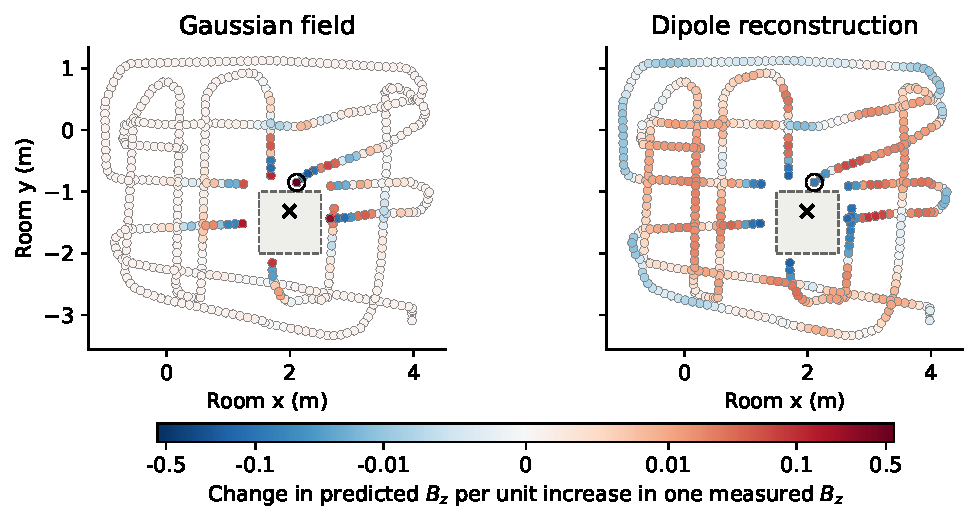
\includegraphics[width=.93\linewidth]{influence_map.pdf}
\par\smallskip
\raggedright\small\textbf{Figure 1.} Each dot is one training reading. Its color gives
the signed change in predicted \(B_z\) when that reading's \(B_z\) increases
by one reference-instrument unit. The common scale is linear near zero
(\(\pm0.01\)) and logarithmic beyond. The cross marks the query, the box the
gap, and the ring the reading with the largest difference between models.
Larger absolute weights are drawn on top.
\end{minipage}

The largest difference in the influence maps (Figure~1) occurs at \((\SampleX,\SampleY)\) m,
just north of the gap. Increasing its \(B_z\) by one gives
\(\Delta\widehat B_z=\KernelChange\) for the Gaussian field and
\(\Delta\widehat B_z=\DipoleChange\) for the dipole field. Refitting both
models after that change reproduces the predicted changes in all three
components within \(10^{-9}\) recording units. Applying the full weights to
the original readings also reproduces both archived prediction vectors to
that tolerance.

The projection also changes the spatial distribution of influence. For vertical
weights \(w_i\), define the share beyond one metre as
\(\sum_{d_i>1\,\mathrm m}|w_i|/\sum_i|w_i|\), with \(d_i\) the distance
from reading \(i\) to the query. That share rises from \(\KernelFar\%\) to
\(\DipoleFar\%\). Total absolute weight rises from \(\KernelMass\) to
\(\DipoleMass\) while the signed sum stays one, so there is more cancellation.
Horizontal readings also enter the dipole prediction. The largest absolute
weight from a single horizontal component to \(B_z\) is \(\CrossMax\).

At this location the physical projection draws more strongly on distant
measurements and reverses the response to one nearby reading. This is a
sensitivity of the fitted prediction to recorded inputs. The map alone
cannot locate the room's sources or establish an accuracy gain at other queries.

\head{6. In what sense is the classical field learned?}
At the same planar query \(\rr_*=(\xx_*,0)\), read each row from left to right.
The left column evaluates the fitted coefficients. The right column substitutes
their dependence on the original readings. Write \(k_{*i}=k_\ell(\xx_*,\xx_i)\)
and \(D_{*j}=D(\rr_*,\mathbf s_j)\).
\[
\begin{array}{l@{\qquad}c@{\quad}c@{\quad}c}
 & \text{Sum over fitted responses} && \text{Sum over training examples}\\[4pt]
\widehat{\B}_K(\xx_*) &
 \displaystyle\overline{\B}+\sum_i k_{*i}\boldsymbol\alpha_i
 &=& \displaystyle\sum_i g_{*i}\bb_i \\[7pt]
\widehat{\B}_D(\rr_*) &
 \displaystyle\widehat{\bb}_0+\sum_j D_{*j}\widehat{\mathbf q}_j
 &=& \displaystyle\sum_i W_i(\rr_*)\bb_i
\end{array}
\]
In the first row, Eq.~\eqref{eq:gauss} supplies one scalar weight per reading.
In the second, Eq.~\eqref{eq:weights} gives \(W_i=\sum_a H_{ai}U_a\):
the reading influences the Gaussian targets through \(H\), and the dipole
fit carries those changes to the query through \(U_a\). Each equality is exact
for fixed settings. The two rows can weight the same reading differently,
as Figure~1 shows. Classical theory supplies the response of each dipole.
What the room measurements teach us is which superposition predicts its field.

{\footnotesize
\textbf{References.}
[1] A. Solin et al., \emph{Modeling and interpolation of the ambient magnetic
field by Gaussian processes}, IEEE Trans.\ Robotics (2018).
\href{https://github.com/AaltoML/magnetic-data}{Data and publication}.
[2] J. R. Landers, \emph{From a learned kernel to a magnetic field} (2026),
\href{../02-kernel-to-magnetostatics/kernel_to_magnetostatics.pdf}{companion experiment}.
[3] C. E. Rasmussen and C. K. I. Williams, \emph{Gaussian Processes for Machine
Learning} (MIT Press, 2006), \href{https://gaussianprocess.org/gpml/chapters/RW2.pdf}{ch.~2, sec.~2.6}.}
\end{document}
